%!TeX root=../sensetop.tex
\chapter[Chapter \thechapter]{}
\lettrine[lraise=0.3]{E}{dward}, having carried his thanks to Colonel Brandon, proceeded with his happiness to Lucy; and such was the excess of it by the time he reached Bartlett's Buildings, that she was able to assure Mrs Jennings, who called on her again the next day with her congratulations, that she had never seen him in such spirits before in her life.

Her own happiness, and her own spirits, were at least very certain; and she joined Mrs Jennings most heartily in her expectation of their being all comfortably together in Delaford Parsonage before Michaelmas. So far was she, at the same time, from any backwardness to give Elinor that credit which Edward \textit{would} give her, that she spoke of her friendship for them both with the most grateful warmth, was ready to own all their obligation to her, and openly declared that no exertion for their good on Miss Dashwood's part, either present or future, would ever surprise her, for she believed her capable of doing any thing in the world for those she really valued. As for Colonel Brandon, she was not only ready to worship him as a saint, but was moreover truly anxious that he should be treated as one in all worldly concerns; anxious that his tithes should be raised to the utmost; and secretly resolved to avail herself, at Delaford, as far as she possibly could, of his servants, his carriage, his cows, and his poultry.

It was now above a week since John Dashwood had called in Berkeley Street, and as since that time no notice had been taken by them of his wife's indisposition, beyond one verbal enquiry, Elinor began to feel it necessary to pay her a visit.—This was an obligation, however, which not only opposed her own inclination, but which had not the assistance of any encouragement from her companions. Marianne, not contented with absolutely refusing to go herself, was very urgent to prevent her sister's going at all; and Mrs Jennings, though her carriage was always at Elinor's service, so very much disliked Mrs John Dashwood, that not even her curiosity to see how she looked after the late discovery, nor her strong desire to affront her by taking Edward's part, could overcome her unwillingness to be in her company again. The consequence was, that Elinor set out by herself to pay a visit, for which no one could really have less inclination, and to run the risk of a tête-à-tête with a woman, whom neither of the others had so much reason to dislike.

Mrs Dashwood was denied; but before the carriage could turn from the house, her husband accidentally came out. He expressed great pleasure in meeting Elinor, told her that he had been just going to call in Berkeley Street, and, assuring her that Fanny would be very glad to see her, invited her to come in.

They walked up stairs in to the drawing-room.—Nobody was there.

<Fanny is in her own room, I suppose,> said he: <I will go to her presently, for I am sure she will not have the least objection in the world to seeing \textit{you}. Very far from it, indeed. \textit{Now} especially there cannot be—but however, you and Marianne were always great favourites. Why would not Marianne come?>

Elinor made what excuse she could for her.

<I am not sorry to see you alone,> he replied, <for I have a good deal to say to you. This living of Colonel Brandon's—can it be true?—has he really given it to Edward?—I heard it yesterday by chance, and was coming to you on purpose to enquire farther about it.>

<It is perfectly true.—Colonel Brandon has given the living of Delaford to Edward.>

<Really!—Well, this is very astonishing!—no relationship!—no connection between them!—and now that livings fetch such a price!—what was the value of this?>

<About two hundred a year.>

<Very well—and for the next presentation to a living of that value—supposing the late incumbent to have been old and sickly, and likely to vacate it soon—he might have got I dare say—fourteen hundred pounds. And how came he not to have settled that matter before this person's death? \textit{Now}, indeed it would be too late to sell it, but a man of Colonel Brandon's sense! I wonder he should be so improvident in a point of such common, such natural, concern! Well, I am convinced that there is a vast deal of inconsistency in almost every human character. I suppose, however—on recollection—that the case may probably be \textit{this}. Edward is only to hold the living till the person to whom the Colonel has really sold the presentation, is old enough to take it. Aye, aye, that is the fact, depend upon it.>

Elinor contradicted it, however, very positively; and by relating that she had herself been employed in conveying the offer from Colonel Brandon to Edward, and, therefore, must understand the terms on which it was given, obliged him to submit to her authority.

<It is truly astonishing!>—he cried, after hearing what she said—<what could be the Colonel's motive?>

<A very simple one—to be of use to Mr Ferrars.>

<Well, well; whatever Colonel Brandon may be, Edward is a very lucky man.—You will not mention the matter to Fanny, however, for though I have broke it to her, and she bears it vastly well,—she will not like to hear it much talked of.>

Elinor had some difficulty here to refrain from observing, that she thought Fanny might have borne with composure, an acquisition of wealth to her brother, by which neither she nor her child could be possibly impoverished.

<Mrs Ferrars,> added he, lowering his voice to the tone becoming so important a subject, <knows nothing about it at present, and I believe it will be best to keep it entirely concealed from her as long as may be. When the marriage takes place, I fear she must hear of it all.>

<But why should such precaution be used? Though it is not to be supposed that Mrs Ferrars can have the smallest satisfaction in knowing that her son has money enough to live upon, for \textit{that} must be quite out of the question; yet why, upon her late behaviour, is she supposed to feel at all? She has done with her son,—she cast him off for ever, and has made all those over whom she had any influence, cast him off likewise. Surely, after doing so, she cannot be imagined liable to any impression of sorrow or of joy on his account: she cannot be interested in any thing that befalls him. She would not be so weak as to throw away the comfort of a child, and yet retain the anxiety of a parent!>

<Ah! Elinor,> said John, <your reasoning is very good, but it is founded on ignorance of human nature. When Edward's unhappy match takes place, depend upon it his mother will feel as much as if she had never discarded him; and, therefore every circumstance that may accelerate that dreadful event, must be concealed from her as much as possible. Mrs Ferrars can never forget that Edward is her son.>

<You surprise me; I should think it must nearly have escaped her memory by \textit{this} time.>

<You wrong her exceedingly. Mrs Ferrars is one of the most affectionate mothers in the world.>

Elinor was silent.

<We think \textit{now},>—said Mr Dashwood, after a short pause, <of \textit{Robert's} marrying Miss Morton.>

Elinor, smiling at the grave and decisive importance of her brother's tone, calmly replied,—

<The lady, I suppose, has no choice in the affair.>

<Choice!—how do you mean?>

<I only mean that I suppose, from your manner of speaking, it must be the same to Miss Morton whether she marry Edward or Robert.>

<Certainly, there can be no difference; for Robert will now to all intents and purposes be considered as the eldest son;—and as to any thing else, they are both very agreeable young men: I do not know that one is superior to the other.>

Elinor said no more, and John was also for a short time silent.—His reflections ended thus.

<Of \textit{one} thing, my dear sister,> kindly taking her hand, and speaking in an awful whisper, <I may assure you;—and I \textit{will} do it, because I know it must gratify you. I have good reason to think—indeed I have it from the best authority, or I should not repeat it, for otherwise it would be very wrong to say any thing about it,—but I have it from the very best authority,—not that I ever precisely heard Mrs Ferrars say it herself—but her daughter \textit{did}, and I have it from her,—that in short, whatever objections there might be against a certain—a certain connection, you understand me,—it would have been far preferable to her,—it would not have given her half the vexation that \textit{this} does. I was exceedingly pleased to hear that Mrs Ferrars considered it in that light; a very gratifying circumstance you know to us all. <It would have been beyond comparison,> she said, <the least evil of the two, and she would be glad to compound \textit{now} for nothing worse.> But however, all that is quite out of the question,—not to be thought of or mentioned—as to any attachment you know, it never could be: all that is gone by. But I thought I would just tell you of this, because I knew how much it must please you. Not that you have any reason to regret, my dear Elinor. There is no doubt of your doing exceedingly well,—quite as well, or better, perhaps, all things considered. Has Colonel Brandon been with you lately?>

\begin{figure}[tbph]
\centering
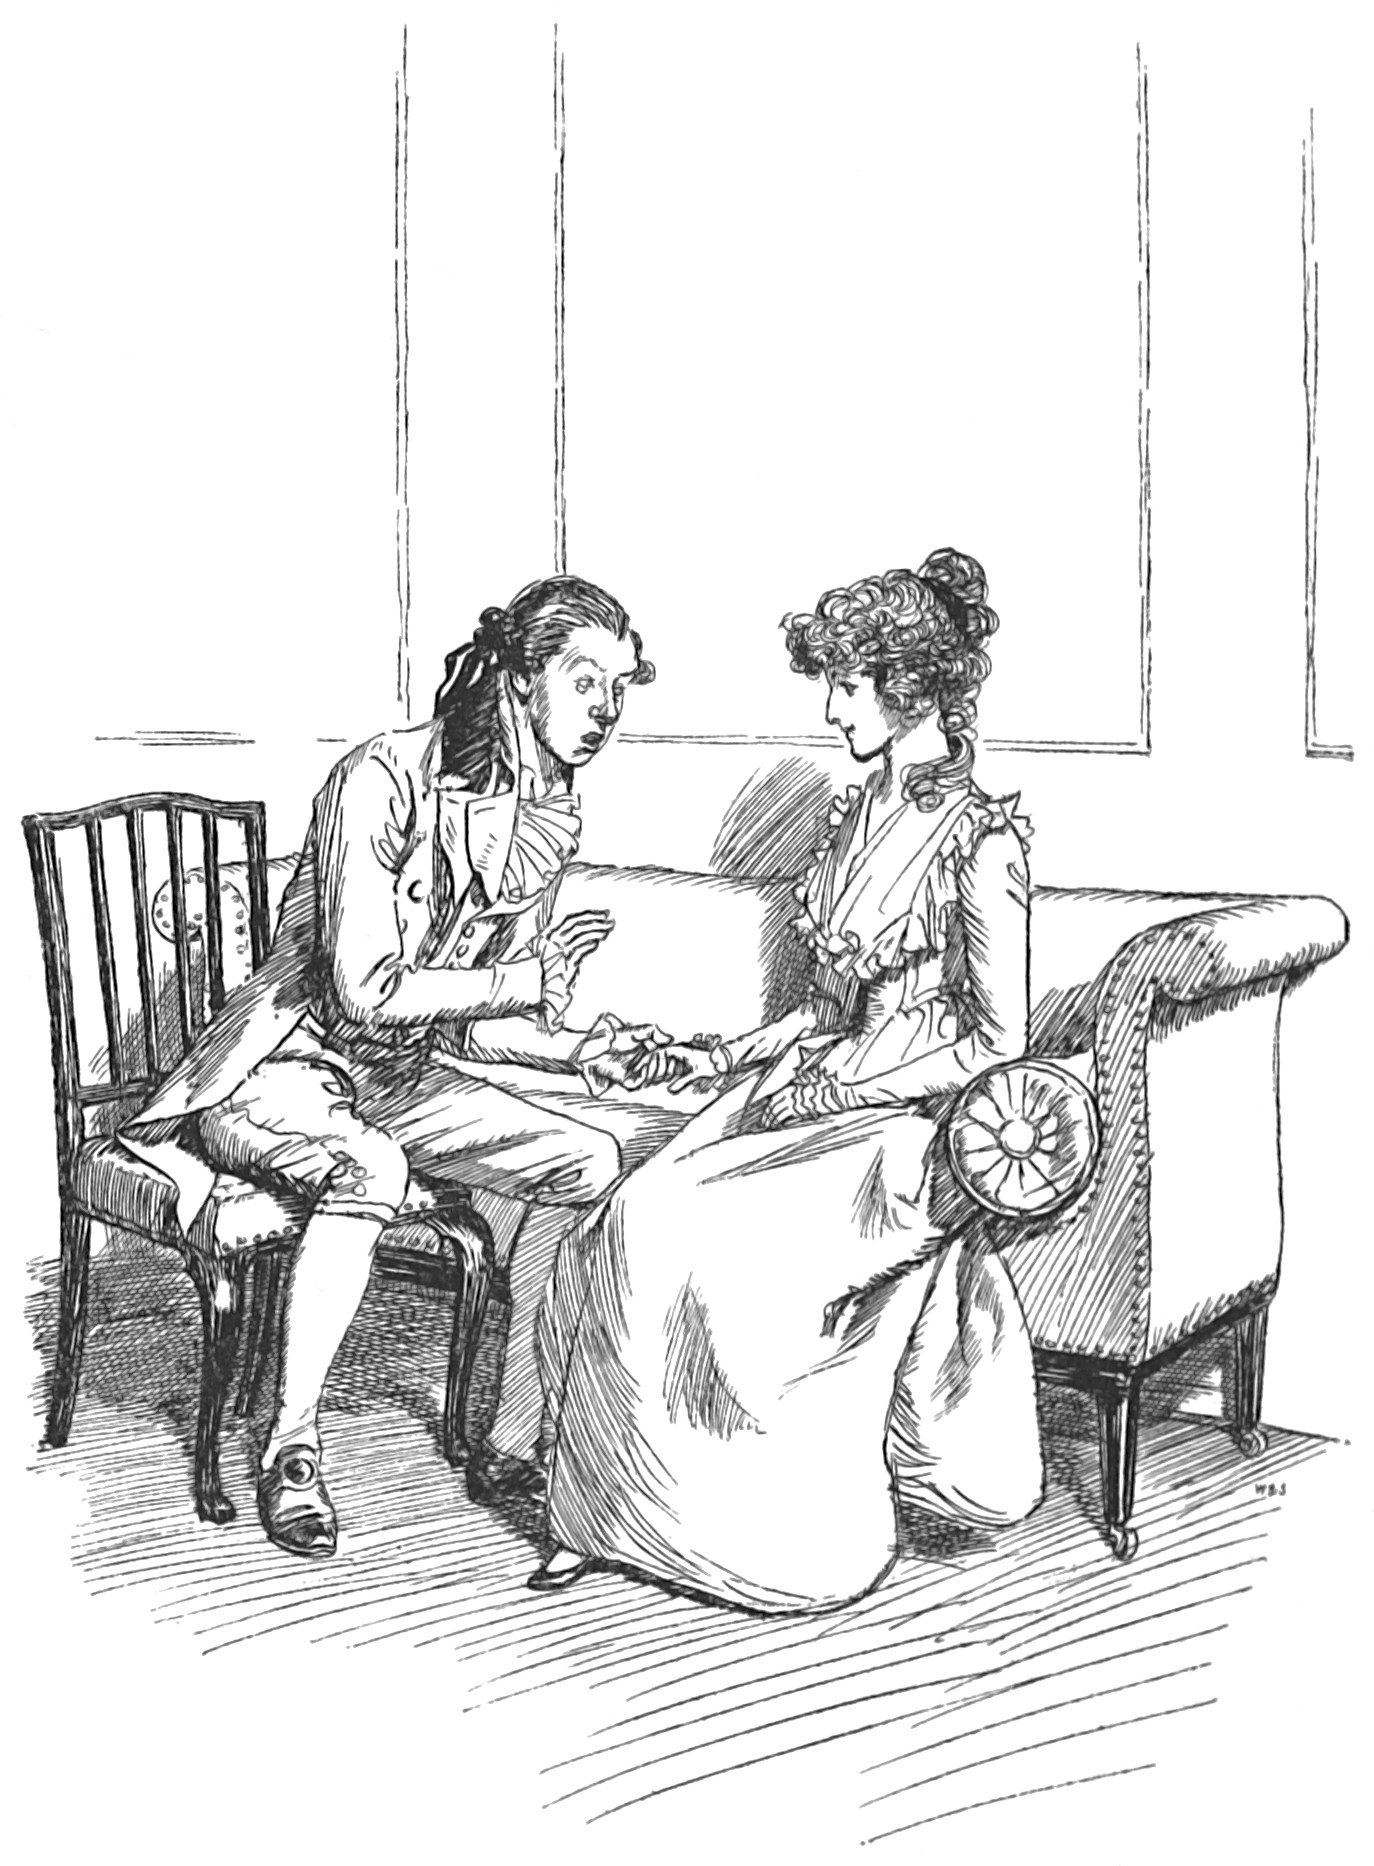
\includegraphics[width=\linewidth]{41assure}
\caption{<Of \textit{one} thing, I may assure you>}
\end{figure}

Elinor had heard enough, if not to gratify her vanity, and raise her self-importance, to agitate her nerves and fill her mind;—and she was therefore glad to be spared from the necessity of saying much in reply herself, and from the danger of hearing any thing more from her brother, by the entrance of Mr Robert Ferrars. After a few moments' chat, John Dashwood, recollecting that Fanny was yet uninformed of her sister's being there, quitted the room in quest of her; and Elinor was left to improve her acquaintance with Robert, who, by the gay unconcern, the happy self-complacency of his manner while enjoying so unfair a division of his mother's love and liberality, to the prejudice of his banished brother, earned only by his own dissipated course of life, and that brother's integrity, was confirming her most unfavourable opinion of his head and heart.

They had scarcely been two minutes by themselves, before he began to speak of Edward; for he, too, had heard of the living, and was very inquisitive on the subject. Elinor repeated the particulars of it, as she had given them to John; and their effect on Robert, though very different, was not less striking than it had been on \textit{him}. He laughed most immoderately. The idea of Edward's being a clergyman, and living in a small parsonage-house, diverted him beyond measure;—and when to that was added the fanciful imagery of Edward reading prayers in a white surplice, and publishing the banns of marriage between John Smith and Mary Brown, he could conceive nothing more ridiculous.

Elinor, while she waited in silence and immovable gravity, the conclusion of such folly, could not restrain her eyes from being fixed on him with a look that spoke all the contempt it excited. It was a look, however, very well bestowed, for it relieved her own feelings, and gave no intelligence to him. He was recalled from wit to wisdom, not by any reproof of hers, but by his own sensibility.

<We may treat it as a joke,> said he, at last, recovering from the affected laugh which had considerably lengthened out the genuine gaiety of the moment; <but, upon my soul, it is a most serious business. Poor Edward! he is ruined for ever. I am extremely sorry for it; for I know him to be a very good-hearted creature; as well-meaning a fellow perhaps, as any in the world. You must not judge of him, Miss Dashwood, from \textit{your} slight acquaintance. Poor Edward! His manners are certainly not the happiest in nature. But we are not all born, you know, with the same powers,—the same address. Poor fellow! to see him in a circle of strangers! To be sure it was pitiable enough; but upon my soul, I believe he has as good a heart as any in the kingdom; and I declare and protest to you I never was so shocked in my life, as when it all burst forth. I could not believe it. My mother was the first person who told me of it; and I, feeling myself called on to act with resolution, immediately said to her, <My dear madam, I do not know what you may intend to do on the occasion, but as for myself, I must say, that if Edward does marry this young woman, \textit{I} never will see him again.> That was what I said immediately. I was most uncommonly shocked, indeed! Poor Edward! he has done for himself completely,—shut himself out for ever from all decent society! But, as I directly said to my mother, I am not in the least surprised at it; from his style of education, it was always to be expected. My poor mother was half frantic.>

<Have you ever seen the lady?>

<Yes; once, while she was staying in this house, I happened to drop in for ten minutes; and I saw quite enough of her. The merest awkward country girl, without style, or elegance, and almost without beauty. I remember her perfectly. Just the kind of girl I should suppose likely to captivate poor Edward. I offered immediately, as soon as my mother related the affair to me, to talk to him myself, and dissuade him from the match; but it was too late \textit{then}, I found, to do any thing, for unluckily, I was not in the way at first, and knew nothing of it till after the breach had taken place, when it was not for me, you know, to interfere. But had I been informed of it a few hours earlier, I think it is most probable that something might have been hit on. I certainly should have represented it to Edward in a very strong light. <My dear fellow,> I should have said, <consider what you are doing. You are making a most disgraceful connection, and such a one as your family are unanimous in disapproving.> I cannot help thinking, in short, that means might have been found. But now it is all too late. He must be starved, you know, that is certain; absolutely starved.>

He had just settled this point with great composure, when the entrance of Mrs John Dashwood put an end to the subject. But though \textit{she} never spoke of it out of her own family, Elinor could see its influence on her mind, in the something like confusion of countenance with which she entered, and an attempt at cordiality in her behaviour to herself. She even proceeded so far as to be concerned to find that Elinor and her sister were so soon to leave town, as she had hoped to see more of them;—an exertion in which her husband, who attended her into the room, and hung enamoured over her accents, seemed to distinguish every thing that was most affectionate and graceful.